%!TEX root = ../dokumentation.tex

%
% Nahezu alle Einstellungen koennen hier getaetigt werden
%

\documentclass[%
	pdftex,
	oneside,		% Einseitiger Druck.
	12pt,			% Schriftgroesse
	parskip=half,	% Halbe Zeile Abstand zwischen Absätzen.
	headsepline,	% Linie nach Kopfzeile.
	footsepline,	% Linie vor Fusszeile.
	abstracton,	    % Abstract Überschriften
	ngerman,		% Translator
]{scrreprt}

%Seitengroesse
\usepackage{fullpage}

%Zeilenumbruch und mehr
\usepackage[activate]{microtype}

% Zeichencodierung
\usepackage[utf8]{inputenc}
\usepackage[T1]{fontenc}

% Zeilenabstand
\usepackage[onehalfspacing]{setspace}

% Index-Erstellung
\usepackage{makeidx}

% Lokalisierung (neue deutsche Rechtschreibung)
\usepackage[ngerman]{babel}

% Anführungszeichen 
\usepackage[babel,german=quotes]{csquotes}
%\usepackage[style=swiss]{csquotes}


% Spezielle Tabellenform fuer Deckblatt
\usepackage{longtable}
\setlength{\tabcolsep}{10pt} %Abstand zwischen Spalten
\renewcommand{\arraystretch}{1.5} %Zeilenabstand

% Grafiken
\usepackage{graphicx}

% Mathematische Textsaetze
%\usepackage{amsmath}
%\usepackage{amssymb}

% Pakete um Textteile drehen zu können, oder eine Seite Querformat anzeigen kann.
%\usepackage{rotating}
%\usepackage{lscape}

% Farben
\usepackage{color}
\definecolor{LinkColor}{rgb}{0,0,0.2}
\definecolor{ListingBackground}{rgb}{0.92,0.92,0.92}
\definecolor{pblue}{rgb}{0.13,0.13,1}
\definecolor{pgreen}{rgb}{0,0.5,0}
\definecolor{pred}{rgb}{0.9,0,0}
\definecolor{pgrey}{rgb}{0.46,0.45,0.48}



\newcommand{\pdftitel}{Grafische Einbindung von Plug-ins im Eclipse Rich Client Platform Umfeld}
\newcommand{\autor}{Max Emmert}
\newcommand{\arbeit}{Praxisbericht}

% Titel, Autor und Datum
\title{\titel}
\author{\autor}
\date{\datum}

% PDF Einstellungen
\usepackage[%
	pdftitle={\pdftitel},
	pdfauthor={\autor},
	pdfsubject={\arbeit},
	pdfcreator={pdflatex, LaTeX with KOMA-Script},
	pdfpagemode=UseOutlines, % Beim Oeffnen Inhaltsverzeichnis anzeigen
	pdfdisplaydoctitle=true, % Dokumenttitel statt Dateiname anzeigen.
	pdflang=de % Sprache des Dokuments.
]{hyperref} 

% (Farb-)einstellungen für die Links im PDF
\hypersetup{%
	colorlinks=true, % Aktivieren von farbigen Links im Dokument
	linkcolor=LinkColor, % Farbe festlegen
	citecolor=LinkColor,
	filecolor=LinkColor,
	menucolor=LinkColor,
	urlcolor=LinkColor,
	bookmarksnumbered=true % Überschriftsnummerierung im PDF Inhalt anzeigen.
}

% Literaturverweise nach Harvard (mit deutschem und)
\usepackage[dcucite]{harvard}
\renewcommand{\harvardand}{und}

% Verschiedene Schriftarten
%\usepackage{goudysans}
%\usepackage{lmodern}
%\usepackage{libertine}
\usepackage{palatino} 

\definecolor{dkgreen}{rgb}{0,0.6,0}
\definecolor{gray}{rgb}{0.5,0.5,0.5}
\definecolor{mauve}{rgb}{0.58,0,0.82}
 \definecolor{middlegray}{rgb}{0.5,0.5,0.5}
 \definecolor{lightgray}{rgb}{0.9,0.9,0.9}
 \definecolor{orange}{rgb}{0.8,0.3,0.3}
 \definecolor{yac}{rgb}{0.6,0.6,0.1}



% Hurenkinder und Schusterjungen verhindern
% http://projekte.dante.de/DanteFAQ/Silbentrennung
\clubpenalty=10000
\widowpenalty=10000
\displaywidowpenalty=10000

% Quellcode
\usepackage{listings}
\lstloadlanguages{Java}

\lstset{language=Java,
  backgroundcolor=\color{lightgray},
  numbers=left,
  stepnumber=1,
  xleftmargin=15pt,
  showspaces=false,
  showtabs=false,
  breaklines=true,
  showstringspaces=false,
  breakatwhitespace=true,
  commentstyle=\color{pgreen},
  keywordstyle=\color{pblue},
  stringstyle=\color{pred},
  basicstyle=\ttfamily,
  moredelim=[il][\textcolor{pgrey}]{$$},
  moredelim=[is][\textcolor{pgrey}]{\%\%}{\%\%}
}

% Glossar
\usepackage[
	nonumberlist, %keine Seitenzahlen anzeigen
	%acronym,      %ein Abkürzungsverzeichnis erstellen
	%section,     %im Inhaltsverzeichnis auf section-Ebene erscheinen
	toc,          %Einträge im Inhaltsverzeichnis
]{glossaries}

%Akronyme
\usepackage[printonlyused,footnote]{acronym}

% Fussnoten
\usepackage[perpage, hang, multiple, stable]{footmisc}

%Bildpfad
\graphicspath{{images/}}

%nur ein latex-Durchlauf für die Aktualisierung von Verzeichnissen nötig
\usepackage{bookmark}

%Gleitumgebungen (Bilder, Tabellen, usw\ldots) lassen sich mit H an genau der
% definierten Stelle platzieren
\usepackage{float}

% für die vertikale Platzierung von Text in Tabellen
\usepackage{array}

% für die Darstellung des Euro-Symbols
\usepackage[right]{eurosym}

% für textumflossene Grafiken
\usepackage{wrapfig}

% eine Kommentarumgebung "k" (Handhabe mit \begin{k}<Kommentartext>\end{k},
% Kommentare werden rot gedruckt). Wird \% vor excludecomment{k} entfernt,
% werden keine Kommentare mehr gedruckt.
\usepackage{comment}
\specialcomment{k}{\begingroup\color{red}}{\endgroup}
%\excludecomment{k}


% Ab jetzt können auch Umlaute verwendet werden

%falls pdftitel = titel der Arbeit
\newcommand{\titel}{\pdftitel}
%bei unterschiedlichen Titeln
%\newcommand{\titel}{In der Regel haben wir einen zweizeiligen
% Bachelorthesistitel}
\newcommand{\martrikelnr}{8132098}
\newcommand{\kurs}{STG-TINF12C}
\newcommand{\datumAbgabe}{März 2014}
\newcommand{\firma}{Compart AG}
\newcommand{\firmenort}{Böblingen}
\newcommand{\abgabeort}{Stuttgart}
\newcommand{\abschluss}{Bachelor of Engineering}
\newcommand{\studiengang}{Angewandte Informatik}
\newcommand{\dhbw}{Stuttgart}
\newcommand{\betreuer}{Lars Heppler}
\newcommand{\zeitraum}{12 Wochen}
\newcommand{\arbeitsart}{\arbeit}

\makeglossaries
%!TEX root = ../dokumentation.tex

%
% vorher in Konsole folgendes aufrufen: 
%	makeglossaries makeglossaries dokumentation.acn && makeglossaries dokumentation.glo
%

%
% Glossareintraege --> referenz, name, beschreibung
% Aufruf mit \gls{...}
%
\newglossaryentry{Glossareintrag}{name={Glossareintrag},plural={Glossareinträge},description={Ein Glossar beschreibt verschiedenste Dinge in kurzen Worten}}

\newglossaryentry{Mockup}{name={Mockup},plural={Mockups},description={Ein Mockup ist ein maßstäbliches Modell, das oft zu Präsentationszwecken oder zur Veranschaulichung genutzt wird}}

\newglossaryentry{Toolbar}{name={Toolbar},plural={Toolbars},description={Eine Toolbar (Statusleiste) ist eine waagerechte oder senkrechte Leiste mit kleinen, häufig bebilderten Schaltflächen, die als erweiternde Elemente der Menüführung von Programmen mit grafischer Benutzeroberfläche dienen}}

\newglossaryentry{String}{name={String},plural={Strings},description={Ein String ist eine Zeichenkette bzw. eine Folge von Zeichen aus einem definierten Zeichensatz}}

\newglossaryentry{Framework}{name={Framework},plural={Frameworks},description={Programmiergerüst, das in der Softwaretechnik im Rahmen der objektorientierten Softwareentwicklung sowie bei komponentenbasierten Entwicklungsansätzen verwendet wird}}

\newglossaryentry{Logging}{name={Logging},plural={Loggings},description={(Automatische) Speicherung von Prozessen und Datenänderungen}}

\newglossaryentry{Plug-in}{name={Plug-in},plural={Plug-ins},description={Erweiterungsmodul, das von einer Software während ihrer Laufzeit erkannt und angeschlossen werden kann. Mit Plug-ins werden Applikationen um zusätzliche Funktionalitäten erweitert}}

\newglossaryentry{Repository}{name={Repository},plural={Repositories},description={Verwaltetes Verzeichnis zur Speicherung und Beschreibung von digitalen Objekten (oft genutzt im Zusammenhang mit Versionsverwaltung)}}

\newglossaryentry{Versionsverwaltung}{name={Versionsverwaltung},plural={Versionsverwaltungen},description={System, das zur Erfassung von Änderungen an Dokumenten oder Dateien verwendet wird. Alle Versionen werden in einem Archiv oder Repository abgelegt, um ungewollte Datenverluste zu vermeiden}}






\begin{document}

	% Deckblatt
	\begin{spacing}{1}
		%!TEX root = ../dokumentation.tex

\begin{titlepage}
	\begin{longtable}{p{.4\textwidth} p{.4\textwidth}}
	  {
\includegraphics[height=1.8cm]{Logo-Compart-96dpi.jpg}} & 
	  {
\includegraphics[height=1.8cm]{images/dhbw.png}}
	\end{longtable}
	\enlargethispage{20mm}
	\begin{center}
	  \vspace*{12mm}	{\LARGE\bf \titel }\\
	  \vspace*{12mm}	{\large\bf \arbeit}\\
	 % \vspace*{12mm}	für die Prüfung zum\\
	 % \vspace*{3mm} 	{\bf \abschluss}\\
	  \vspace*{12mm}	des Studiengangs \studiengang\\
	  \vspace*{3mm} 	an der Dualen Hochschule Baden-Württemberg \dhbw\\
	  \vspace*{12mm}	von\\
	  \vspace*{3mm} 	{\large\bf \autor}\\
	  \vspace*{12mm}	\datumAbgabe\\
	\end{center}
	\vfill
	\begin{spacing}{1.2}
	\begin{tabbing}
		mmmmmmmmmmmmmmmmmmmmmmmmmm     \= \kill
	%	\textbf{Bearbeitungszeitraum}  \>  \zeitraum\\
		\textbf{Matrikelnummer, Kurs}  \>  \martrikelnr, \kurs\\
		\textbf{Ausbildungsfirma}      \>  \firma, \firmenort\\
		\textbf{Betreuer}              \>  \betreuer\\
	\end{tabbing}
	\end{spacing}
\end{titlepage}

	\end{spacing}
	\newpage

	\renewcommand{\thepage}{\Roman{page}}
	\setcounter{page}{1}

	% Sperrvermerk
	%!TEX root = ../dokumentation.tex

\thispagestyle{empty}
% Sperrvermerk direkt hinter Titelseite
\section*{Sperrvermerk}

\vspace*{2em}

Die vorliegende {\arbeitsart} mit dem Titel {\itshape \titel} ist mit einem Sperrvermerk versehen und wird ausschließlich zu Prüfungszwecken am Studiengang {\studiengang} der Dualen Hochschule Baden-Württemberg {\abgabeort} vorgelegt.
Jede Einsichtnahme und Veröffentlichung – auch von Teilen der Arbeit – bedarf der vorherigen Zustimmung durch die {\firma}.

	\newpage
	
	% Erklärung
	%!TEX root = ../dokumentation.tex

\thispagestyle{empty}

\section*{Erklärung}
% http://www.se.dhbw-mannheim.de/fileadmin/ms/wi/dl_swm/dhbw-ma-wi-organisation-bewertung-bachelorarbeit-v2-00.pdf
\vspace*{2em}

Ich erkläre hiermit ehrenwörtlich: \\
\begin{enumerate}
\item dass ich meinen {\arbeitsart} mit dem Thema
{\itshape \titel } ohne fremde Hilfe angefertigt habe;
\item dass ich die Übernahme wörtlicher Zitate aus der Literatur sowie die Verwendung der Gedanken
anderer Autoren an den entsprechenden Stellen innerhalb der Arbeit gekennzeichnet habe;
\item dass ich meine {\arbeitsart} bei keiner anderen Prüfung vorgelegt habe;
%\item dass die eingereichte elektronische Fassung exakt mit der eingereichten %schriftlichen Fassung
%übereinstimmt.
\end{enumerate}

Ich bin mir bewusst, dass eine falsche Erklärung rechtliche Folgen haben wird.

\vspace{3em}

\abgabeort, \datumAbgabe
\vspace{4em}

\autor

	\newpage

	% Abstract
	%!TEX root = ../dokumentation.tex

\pagestyle{empty}

\renewcommand{\abstractname}{Zusammenfassung}
\begin{abstract}
Ein Abstract ist eine prägnante Inhaltsangabe, ein Abriss ohne
Interpretation und Wertung einer wissenschaftlichen Arbeit. In DIN
1426 wird das (oder auch der) Abstract als Kurzreferat zur
Inhaltsangabe beschrieben.

\begin{description}
\item[Objektivität] soll sich jeder persönlichen Wertung enthalten
\item[Kürze] soll so kurz wie möglich sein
\item[Genauigkeit] soll genau die Inhalte und die Meinung der Originalarbeit wiedergeben
\end{description}

Üblicherweise müssen wissenschaftliche Artikel einen Abstract
enthalten, typischerweise von 100-150 Wörtern, ohne Bilder und
Literaturzitate und in einem Absatz.

Quelle \url{http://de.wikipedia.org/wiki/Abstract} Abgerufen 07.07.2011
\end{abstract}


\renewcommand{\abstractname}{Summary}
\begin{abstract}
An abstract is a brief summary of a research article, thesis, review,
conference proceeding or any in-depth analysis of a particular subject
or discipline, and is often used to help the reader quickly ascertain
the paper's purpose. When used, an abstract always appears at the
beginning of a manuscript, acting as the point-of-entry for any given
scientific paper or patent application. Abstracting and indexing
services for various academic disciplines are aimed at compiling a
body of literature for that particular subject.

The terms précis or synopsis are used in some publications to refer to
the same thing that other publications might call an "abstract". In
management reports, an executive summary usually contains more
information (and often more sensitive information) than the abstract
does.

Quelle: \url{http://en.wikipedia.org/wiki/Abstract_(summary)}

\end{abstract}

	\newpage

	\pagestyle{plain}

	% Inhaltsverzeichnis
	\begin{spacing}{1.1}
		\setcounter{tocdepth}{1}
		%für die Anzeige von Unterkapiteln im Inhaltsverzeichnis
		%\setcounter{tocdepth}{2}
		\tableofcontents
	\end{spacing}
	\newpage

	\renewcommand{\thepage}{\arabic{page}}
	\setcounter{page}{1}
	
	% Inhalt
	%!TEX root = ../dokumentation.tex

\chapter{Einleitung}
\label{cha:Einleitung}

\section{Motivation}{
Noch vor einigen Jahren war es nicht unüblich, Anwendungen über die Kommandozeile zu steuern. Die funktionalen Aspekte einer Anwendung hatten eine höhere Priorität als ihre Nutzbarkeit. Um komplizierte Applikationen über die Kommandozeile zu bedienen ist jedoch oft Expertenwissen notwendig. Deshalb spielt die Entwicklung von grafischen Oberflächen in der heutigen Anwendungsentwicklung eine immer größere Rolle. Es reicht oft nicht aus, dem Benutzer nur eine grafische Möglichkeit zur Steuerung einer Applikation zu geben. Im Rahmen der Software-Ergonomie spielt die Benutzerführung eine tragende Rolle. So auch bei der Anwendung Workbench for Mill Plus, eine Anwendung der Compart AG, die es dem Anwender ermöglicht bequem Prozesse zur Modifikation und Konvertierung von Dokumenten zu steuern. Der Anwendung Workbench for Mill Plus liegt die Programmiersprache Java zu Grunde. Durch die hohe Verbreitung von Java entstehen immer komplexere Anwendungen. Um die Komplexität solcher Anwendungen handhaben zu können bedient man sich oft Mitteln zur Modularisierung. Hierfür hat Java jedoch keine eigene Sprachunterstützung. \ac{OSGi} bietet die Möglichkeit, monolithischen Anwendungen, die den heutigen dynamischen Anforderungen nicht gerecht werden, entgegenzuwirken.
}
\section{Zielsetzung}{
In der vorausgegangenen Praxisphase wurde vom Studenten ein Programm entwickelt, das es ermöglicht Filterprofile anhand eines gegebenen XML-Schemas zu aktualisieren. Diese Funktionalität soll nun in die DocBridge Workbench for Mill Plus integriert werden. Dies würde Kunden bei der Auslieferung eines neuen XML-Schemas die Möglichkeit geben, die Konfiguration ihrer alten Profile beizubehalten beziehungsweise ein neues Filterprofil zu erstellen, das die Konfiguration des alten Filterprofils enthält, jedoch zum neuen XML-Schema valide ist. Darüber hinaus soll es dem Anwender möglich sein, Profile in die DocBridge Workbench for Mill Plus zu importieren. Wird beim Import festgestellt, dass das Filterprofil nicht dem gegebenen XML-Schema entspricht soll dies dem Anwender kenntlich gemacht werden. 
}
\section{Aufbau der Arbeit}{Die \nameref{cha:Einleitung} soll dem Leser einen Überblick über das Thema verschaffen. Es werden sowohl die Motivation hinter dieser Arbeit als auch deren Zielsetzung abgehandelt. Das Kapitel \nameref{cha:Grundlagen} soll dem Leser einen Überblick über das Thema verschaffen. Es werden die Motivation und die Zielsetzung dieser Arbeit erläutert. Darüber hinaus werden Begriffe und Systeme erklärt, die für das Verständnis und Nachvollziehbarkeit der Arbeit grundlegend sind. Im \nameref{cha:Hauptteil} wird die Vorgehensweise zur Problemlösung detailliert beschrieben. Er umfasst die \nameref{sec:analyse} der zugrunde liegenden Thematik ebenso wie das \nameref{sec:konzept} zur Lösung der behandelten Aufgabe. Die Umsetzung wird im Abschnitt \nameref{sec:implementierung} beschrieben. Im Abschluss daran wird auf die \nameref{sec:ergebnisse} der Arbeit eingegangen. 
}

	%!TEX root = ../dokumentation.tex

\chapter{Grundlagen}
\label{cha:Grundlagen}

\section{DocBridge Mill Plus}{
\label{sec:MillPlus}
DocBridge Mill Plus ist eine plattformunabhängige, skalierbare Software für die Anzeige und Verarbeitung von Datenströmen. Sie ermöglicht die Analyse und Modifikation von Dokumenten in verschiedensten Formaten und die Konvertierung in unterschiedliche Ausgangsformate. Die Dokumente lassen sich auf nahezu allen gängigen physikalischen und digitalen Kanälen darstellen. Mit DocBridge Mill Plus ist der Anwender auch in der Lage Prozesse, die im Output-Management üblich sind, abzubilden. Der modulare Aufbau der Software lässt es zu, sie mit zusätzlichen Modulen um Ein-und Ausgabeformate und Workflows zu erweitern.

\begin{figure}[htbp] 
  \centering
     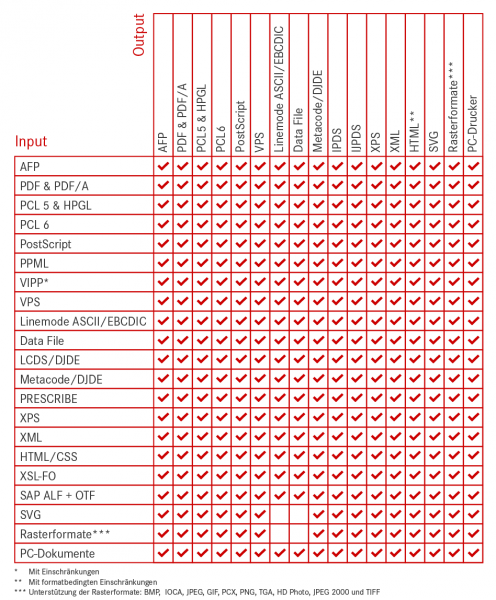
\includegraphics[height=.6\textwidth]{compart_matrix_de.png}
  \caption{Mögliche Verarbeitungsformate der DocBridge Mill Plus}
  \label{fig:compart_matrix}
\end{figure}

\newpage

}

\section{DocBridge Workbench for Mill Plus}{
\label{sec:DBWB}
DocBridge Workbench for Mill Plus bietet eine grafische Benutzeroberfläche für die Filterkonfiguration und die formatunabhängige Dokumentendarstellung. In der \ac{DBWB} können einzelne, mehrere oder in Stapeln zusammengefasste Dokumente angezeigt werden. Es werden alle in Abbildung \ref{fig:compart_matrix} aufgeführten Formate unterstützt. Geladene Dokumente können in der, in Abbildung \ref{fig:dbwb_document} vorgestellten Dokumentenperspektive einheitlich dargestellt werden. Alle Dokumente, die in einem der unterstützten Formaten vorliegen, können im Anzeigebereich untersucht werden. So ist es dem Nutzer möglich, sich unabhängig vom Format des Dokuments, völlig auf dessen Inhalt des zu konzentrieren. In der Prozessperspektive (Abbildung \ref{fig:dbwb_process}) können Verarbeitungsschritte konfiguriert, validiert und lokal ausgeführt werden. Die erstellte Prozesskonfiguration kann exportiert und in der DocBridge Mill Plus ausgeführt werden. Die Konfiguration der Prozesse erfolgt überwiegend über Drag \& Drop. Die Prozessperspektive ist die Standartperspektive der \ac{DBWB}.     

\newpage

\begin{figure}[htbp] 
\centering
     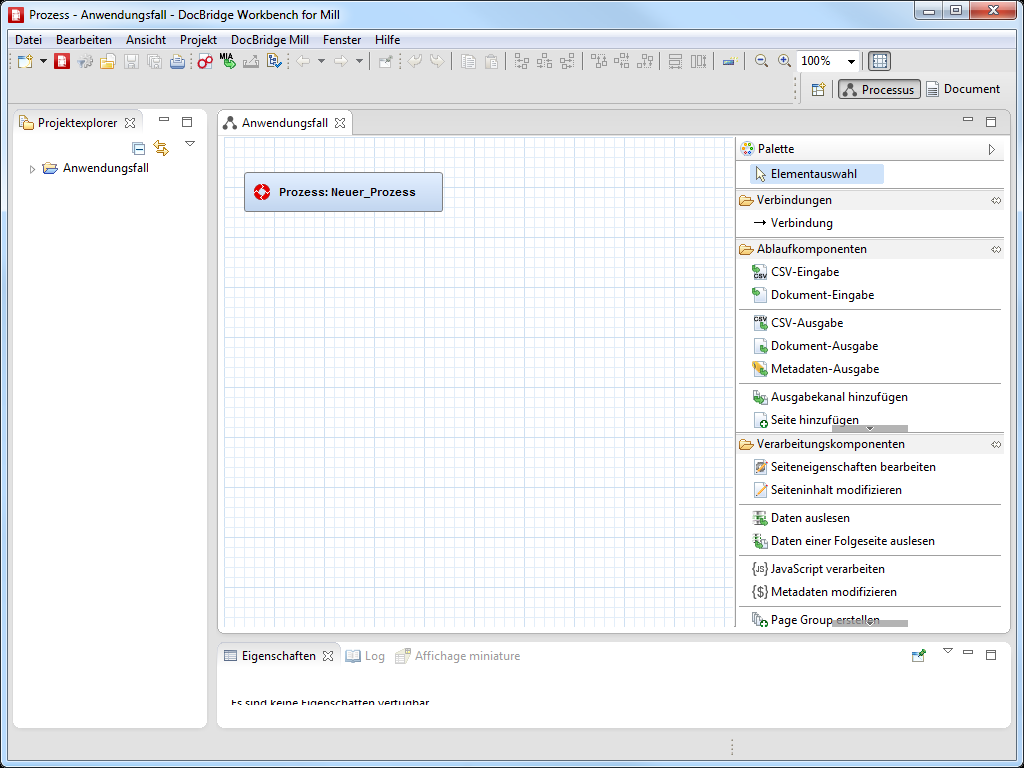
\includegraphics[height=.46\textwidth]{dbwb_process.png}
  \caption{Prozessperspektive}
  \label{fig:dbwb_process}
\end{figure}

\begin{figure}[htbp] 
\centering
     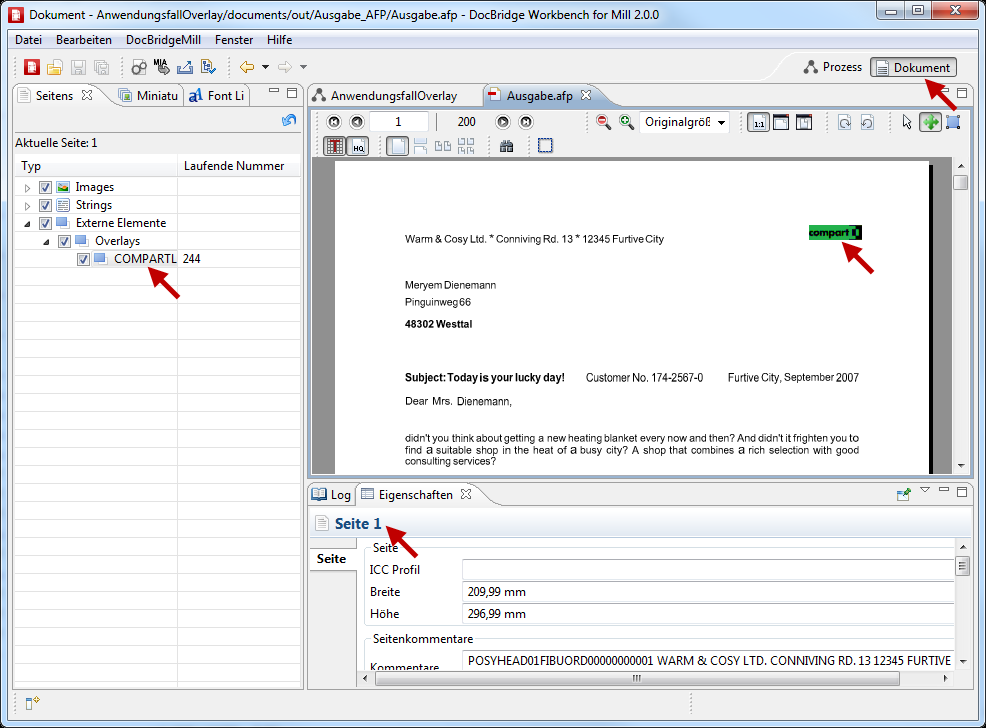
\includegraphics[height=.46\textwidth]{dbwb_document.png}
  \caption{Dokumentperspektive}
  \label{fig:dbwb_document}
\end{figure}


}
\newpage

\section{OSGi}{
\label{sec:OSGi}
\ac{OSGi} Services ermöglichen die Zusammenarbeit einzelner Bundles. Java stellt nur begrenzte Möglichkeiten zur Modularisierung bereit. Java Klassen lassen sich zwar unter der Verwendung von Packages gruppieren, jedoch ist es nicht möglich diese Gruppierungen und Restriktionen zur Laufzeit beizubehalten. Die Möglichkeit, einzelne Klassen als package-protected zu deklarieren ist meist keine befriedigende Lösung. \ac{OSGi} ermöglicht die Verwaltung der Sichtbarkeit von Packages zur Laufzeit. \ac{OSGi} ist ein Framework, welches sich auch dem Problem der Modularisierung annimmt und die Entwicklung von modularen Anwendungen auf der Java-Plattform ermöglicht, was in Abbildung \ref{fig:osgi_layer} veranschaulicht wird. \ac{OSGi}-Anwendungen bestehen aus einzelnen Modulen, die auch Bundles genannt werden. Jedes Bundle hat einen eigenen Lebenszyklus. Dies bedeutet, dass zur Laufzeit einzelne Bundles dynamisch geladen und entfernt werden können. Die Spezifikation von \ac{OSGi} wird von der \ac{OSGi} Alliance erstellt. Die \ac{OSGi} Alliance wurde 1999 von rund 30 namhaften Firmen gegründet, um den Anforderungen im Bereich der eingebetteten Systeme gerecht zu werden. \cite[S.3]{Queue} Die Eclipse \ac{IDE} arbeitet seit Version 3.0 mit der \ac{OSGi} Implementierung Equinox.  

\begin{figure}[htbp] 
\centering
     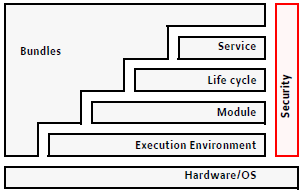
\includegraphics[height=.5\textwidth]{osgi_layer.png}
  \caption{OSGi Schichtenmodell \protect  \cite[aus S.2]{OSGi}}
  \label{fig:osgi_layer}
\end{figure}

}


\section{OSGi Services}{
\label{sec:OSGi_Services}
Bei \ac{OSGi} Services handelt es sich um Java-Objekte, die unter einem Interface in der \ac{OSGi} Service-Registry angemeldet werden. In der Service-Registry angemeldete Services können von anderen Bundles verwendet werden. Services können genau wie OSGi-Bundles dynamisch geladen und entfernt werden. Wird ein Bundle, das einen Service bereitstellt gestoppt, so muss das verwendende Bundle auf das Wegfallen des Service entsprechend reagieren. \cite[vgl.S.114]{OSGi}
}

\section{SWT}{
\label{sec:SWT}
Das \ac{SWT}  stellt das Framework für grafische Oberflächen auf der Eclipse-Plattform bereit. \ac{SWT} stellt eine Java Schnittstelle für die nativen GUI-Bibliotheken verschiedener Betriebssysteme zur Verfügung. Hierzu gehören Microsoft Windows, Linux\footnote{GIMP Toolkit} und Mac OS X\footnote{Cocoa}. Da auf die spezifischen Steuerelemente des jeweiligen Betriebssystems zugegriffen wird, kann mit SWT auf den oben genannten Plattformen ein natives Aussehen und Verhalten erzielt werden, wie in Abbildung \ref{fig:swt_plattform} veranschaulicht wird.


\begin{figure}[htbp] 
  \centering
     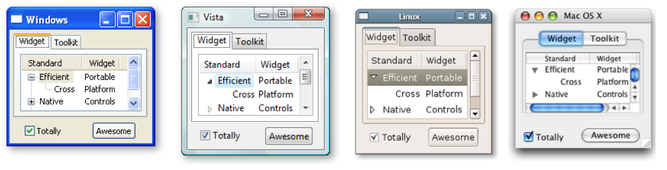
\includegraphics[height=.25\textwidth]{swt_plattform.png}
  \caption{Darstellung von SWT-Widgets auf verschiedenen Betriebssystemen\footnotemark}
   \label{fig:swt_plattform}
\end{figure}
\footnotetext{aus \cite{RalfEbert}}




}

\section{Eclipse RCP}{
\label{sec:Eclipse_rcp}
Eclipse \ac{RCP} ist eine Plattform zur Entwicklung von Desktop-Anwendungen. Sie entstand aus der Eclipse \ac{IDE}, die sich aufgrund ihrer allgemeinen Natur anbietet. Das Eclipse \ac{RCP} Grundgerüst kann durch eigene Anwendungsfunktionalitäten erweitert werden. Viele der vorhandenen Komponenten können in eigenen Anwendungen im Workbench- Aufbau genutzt werden. Als Beispiel wären hier Komponenten für eine Hilfe-Funktion oder das erweiterbare Plug-in-System zu nennen. Vorteile der Anwendungsentwicklung mit Hilfe von Eclipse \ac{RCP} sind Grundstrukturen für den Aufbau von GUI-Anwendungen und der modulare Aufbau. Dieser ermöglicht es, dass Erweiterungen auf Eclipse \ac{RCP} Basis miteinander harmonieren. Die zum implementieren benötigten Werkzeuge sind bereits in der Eclipse \ac{IDE} (Eclipse for RCP/Plug-in Developers)bereits enthalten.
}

\section{Target Platform}{
Eclipse \ac{RCP} Applikationen werden für eine konfigurierbare Zielplattform\footnote{Target Platform} entwickelt. Alle externen Abhängigkeiten werden über die Target Platform geladen. Soll mit Plug-ins die Eclipse \ac{IDE} selbst erweitert werden, verwendet man die standardmäßig die Eclipse \ac{IDE} selbst als Target Platform. \cite[vgl.S14]{RalfEbert} Bei der Entwicklung einer eigenen Rich Client Platform, oder Plug-ins für eine solche, ist es nötig eine eigene Target Platform zu nutzen, da sonst alle Plug-ins und Funktionalitäten der Standard Eclipse IDE auch in der eigenen Applikation wiederzufinden wären. Durch die Definition der Target Platform kann festgelegt werden, in welcher Version der Applikation bestimmte Plug-ins eingebunden werden. Im Idealfall arbeiten alle Entwickler eines Projekts mit der selben Target Platform. So wird eine einheitliche Entwicklungsumgebung sichergestellt.
}

\section{Plug-in zur Profilkonvertierung}{
Vom Studierenden wurde während der letzten Praxiseinheit ein Plug-in im \ac{OSGi}-Umfeld entwickelt, welches dazu verwendet werden kann Filterprofile zu aktualisieren. Die Konfiguration von Konvertierungsabläufen wird in Filterprofilen festgehalten. Deren Aufbau ist in einem XML-Schema definiert. Kommen Funtionalitäten oder Komponenten hinzu, wird das Schema aktualisiert und somit abgeändert. Bestehende Filterprofile sind nun nicht mehr zum Schema valide. Das Plug-in zur Profilkonvertierung liest die Informationen aus dem alten Profil mit Hilfe von verschiedenen Java \ac{API}s aus und generiert anhand des Schemas ein neues Profil, das zum Schema valide ist. Es kommen vor allem die \ac{API}s  Jsoup\footnote{API zum Arbeiten mit degeneriertem HTML} und JaxB\footnote{API für das Erstellen von Klassen aus einer XML-Schema-Instanz} zur Verwendung.
}


	\input{content/03kapitel}
	
	% Anhang
	\clearpage
	\pagenumbering{roman}

	% Abbildungsverzeichnis
	\cleardoublepage
	\phantomsection \label{listoffig}
	\addcontentsline{toc}{chapter}{Abbildungsverzeichnis}
	\listoffigures

	%Tabellenverzeichnis
	\cleardoublepage
	\phantomsection \label{listoftab}
	\addcontentsline{toc}{chapter}{Tabellenverzeichnis}
	\listoftables

	% Quellcodeverzeichnis
	\cleardoublepage
	\phantomsection \label{listoflist}
	\addcontentsline{toc}{chapter}{Listings}
	\lstlistoflistings

	% Literaturverzeichnis
	\cleardoublepage
	\phantomsection \label{listoflit}
	\addcontentsline{toc}{chapter}{Literaturverzeichnis}
	
	%Bib style
	\bibliographystyle{agsm} %Havard
	%\bibliographystyle{amsplain} %Durchnummeriert
	%\bibliographystyle{amsalpha} %Kürzel für Autor und Jahr
	%see more: http://amath.colorado.edu/documentation/LaTeX/reference/faq/bibstyles.pdf
	
	\bibliography{ArbeitBib}

	% Abkürzungsverzeichnis
	\cleardoublepage
	\phantomsection \label{listofacs}
	\addcontentsline{toc}{chapter}{Abkürzungsverzeichnis}
	%!TEX root = ../dokumentation.tex

\chapter*{Abkürzungsverzeichnis}
%nur verwendete Akronyme werden letztlich im Dokument angezeigt
\begin{acronym}[YTMMM]
\setlength{\itemsep}{-\parsep}

\acro{IDE}{Integrierte Entwicklungsumgebung}
\acro{RCP}{Rich Client Platform}
\acro{API}{Application Programming Interface}
\acro{WYSIWYG}{What You See Is What You Get}
\acro{OSGi}{Open Services Gateway initiative}
\acro{SWT}{Standart Widget Toolkit}
\acro{DBWB}{DockBridge Workbench}
\acro{GUI}{Graphical User Interface}
\acro{AFP}{Apple Filing Protocol}
\acro{PDF}{Portable Document Format}
\acro{XML}{Extensible Markup Language}
\acro{HTML}{Hypertext Markup Language}
\acro{XHTML}{Extensible Hypertext Markup Language}
\acro{JRE}{Java Runtime Environment}
\acro{MVC}{Model View Controller}
\acro{SAX}{Simple API for XML}
\acro{DOM}{Document Object Model}
\acro{ASE}{Apache Software Foundation}
\acro{JaxB}{Java Architecture for XML Binding}
\end{acronym}

	
	% Glossar
	\printglossary[style=altlist,title=Glossar]
\end{document}
